      
               
                \begin{ledgroupsized}[r]{120mm}
                \footnotesize 
                \pstart                
                \noindent\textbf{\"{U}berlieferung:}   
                \pend
                \end{ledgroupsized}
            
              
                            \begin{ledgroupsized}[r]{114mm}
                            \footnotesize 
                            \pstart \parindent -6mm
                            \makebox[6mm][l]{\textit{L}}Konzept: LH XXXVIII Bl. 19\textendash 20. 1 Bog. 4\textsuperscript{o}. 3/4 S auf Bl. 20~v\textsuperscript{o}. Die Textpassage im unteren Viertel der Seite zu N. 13\protect\raisebox{-0.5ex}{\tiny{1}} geh\"{o}rig. Die \"{u}brigen Seiten N. 13\protect\raisebox{-0.5ex}{\tiny{1}} und N. 13\protect\raisebox{-0.5ex}{\tiny{3}}. Vgl. dazu die \"{U}berlieferung zu N. 13\protect\raisebox{-0.5ex}{\tiny{1}}. \pend
                            \end{ledgroupsized}
              
                            \begin{ledgroupsized}[r]{114mm}
                            \footnotesize 
                            \pstart \parindent -6mm
                            \makebox[6mm][l]{\textit{E}}\cite{00243}\textsc{Gerland} 1906, S.~199\textendash200.\\Cc 2, Nr. 477 tlw. \pend
                            \end{ledgroupsized}
                \vspace*{8mm}
                \pstart 
                \normalsize
            [20 v\textsuperscript{o}] Collocentur [tres]\edtext{}{\Afootnote{duae\textit{\ L \"{a}ndert Hrsg. } }} rotae\protect\index{Sachverzeichnis}{rota} in navi\protect\index{Sachverzeichnis}{navis}, flexum ejus designaturae, altera  in prora, altera in puppi, tertia in medio. Si navis\protect\index{Sachverzeichnis}{navis} flectitur in medio, correspondent flexus  extremarum rotarum, si in extremis aut inter extrema differunt,  et ex ratione differentiae determinari potest punctum navis\protect\index{Sachverzeichnis}{navis} in quo  facta est flexio. Ne perturbent fluctus inaequales  corresponsum rotarum\protect\index{Sachverzeichnis}{rota}, complicari ita possunt inter se,  ut non possint moveri nisi correspondenter. Cum tamen fluctus inordinati non impingant correspondenter, quod fiet, si aliae rotae\protect\index{Sachverzeichnis}{rota} similes his subjiciantur, sufficiunt vel duae rotae\protect\index{Sachverzeichnis}{rota}. \edtext{In eo difficultas, quod quando jactatur navis, saepe fit ut convertatur  modo in ortum modo in occasum. Hinc remedium istud non sufficit.}{\lemma{rotae.}\Afootnote{ \textit{ (1) }\ Efficiendum est tres rotas\protect\index{Sachverzeichnis}{rota|textit} semper moveri, ut quanto minus mota movetur  tardius magis \textit{ (2) }\ In [...] jactatur \textit{(a)}\ acus \textit{(b)}\ navis, [...] in \textit{(aa)}\ septentrio \textit{(bb)}\ ortum [...] sufficit. \textit{ L}}}  Si centrum sit medium aequalis est celeritas\protect\index{Sachverzeichnis}{celeritas} duarum rotarum\protect\index{Sachverzeichnis}{rota}.  Si centrum est extra medium inaequalis est celeritas\protect\index{Sachverzeichnis}{celeritas}, si centrum est \edtext{in altero extremorum}{\lemma{est}\Afootnote{ \textit{ (1) }\ extra medium \textit{ (2) }\ in altero extremorum \textit{ L}}} quanto magis distat rota\protect\index{Sachverzeichnis}{rota},  tanto circumagetur celerius; nota: ducendus est arcus circuli minoris  in arcum circuli magni seu cujus centrum navis\protect\index{Sachverzeichnis}{navis}, quatenus eum contingit, productum est motus rotae\protect\index{Sachverzeichnis}{rota}.  \pend
            \newpage
            %\begin{wrapfigure}{l}{0.4\textwidth} 
              \begin{center}
              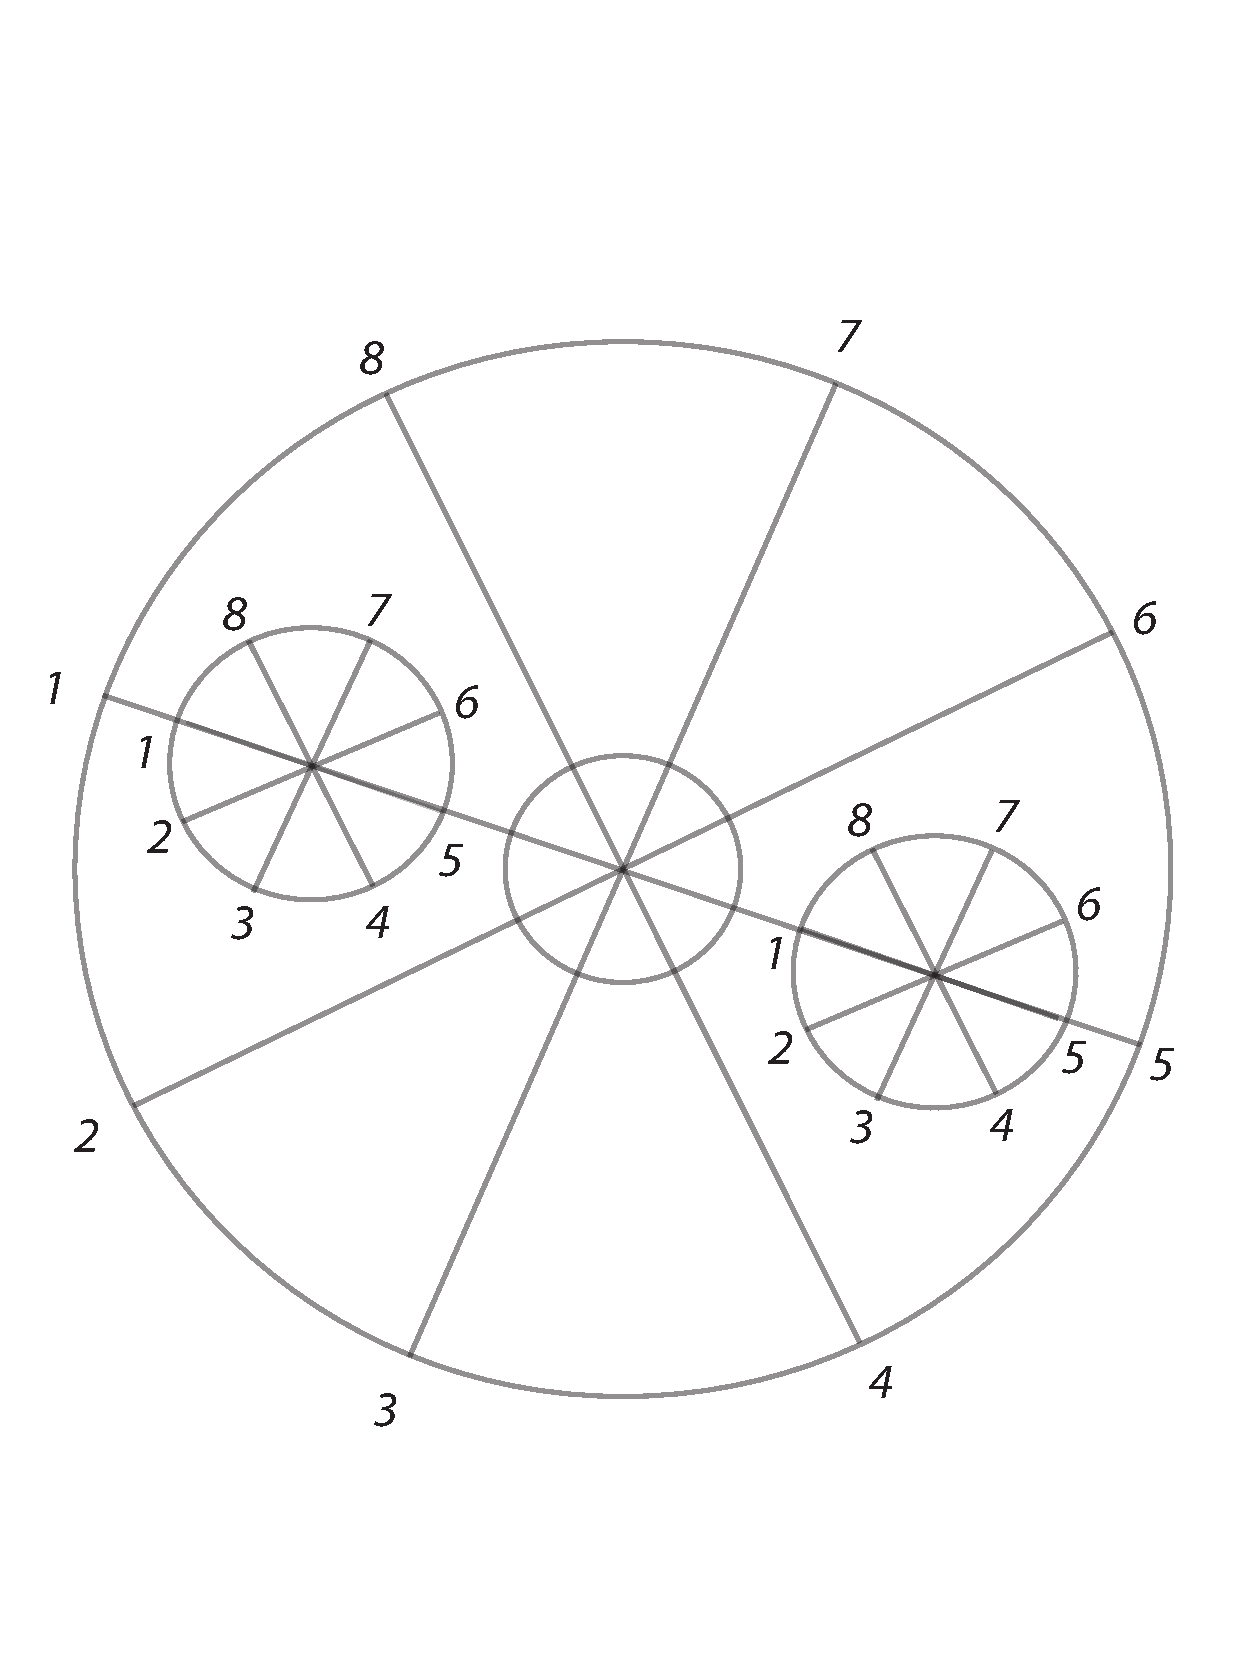
\includegraphics[width=0.6\textwidth]{images/38_20v}
           %  \caption{Bildbeschreibung}
              \\\textit{[Fig. 1, tlw. Blindzeichnung]}
              \end{center}
              %\end{wrapfigure}